\documentclass[11pt]{cernrep} \usepackage{graphicx,epsfig} \bibliographystyle{lesHouches}
\usepackage{xspace}
\newcommand{\Sherpa}{S\protect\scalebox{0.8}{HERPA}\xspace}
\newcommand{\CSS}{C\protect\scalebox{0.8}{SS}\xspace}
\newcommand{\Comix}{C\protect\scalebox{0.8}{OMIX}\xspace}
\newcommand{\Amegic}{A\protect\scalebox{0.8}{MEGIC++}\xspace}
\newcommand{\MCatNLO}{M\protect\scalebox{0.8}{C}@N\protect\scalebox{0.8}{LO}\xspace}
\newcommand{\MEPS}{M\scalebox{0.8}{E}P\scalebox{0.8}{S}\xspace}
\newcommand{\MEPSatNLO}{M\scalebox{0.8}{E}P\scalebox{0.8}{S}@N\protect\scalebox{0.8}{LO}\xspace}
\newcommand{\Collier}{C\protect\scalebox{0.8}{OLLIER}\xspace}
\newcommand{\OpenLoops}{O\protect\scalebox{0.8}{PEN}L\protect\scalebox{0.8}{OOPS}\xspace}

\begin{document}

\section{Study of associated production of vector bosons and b-jets in
  pp collisions at the LHC \protect\footnote{Contributing authors:
    M.~Bell, J.~Butterworth,  V.~Ciulli,
    G.~Hesketh, F. ~Krauss, G.~Luisoni, G.~Nail, D.~Napoletano,
    C.~Oleari, S.~Platzer, C.~Reuschle, B.~Waugh, ... }}

\subsection{Introduction}

\subsection{Event generators}

\subsubsection{Results with \protect\Sherpa }
In this section we present results obtain with the \Sherpa event generator~\cite{Gleisberg:2008ta}. In particular we consider three different classes of samples: 4F~\MCatNLO, 5F~\MEPS and a 5F~\MEPSatNLO one.
\begin{itemize}
\item[4F \MCatNLO : ]{
	This first set of results is obtained in the four-flavour scheme, and based
	on the \MCatNLO technique~\cite{Frixione:2002ik}, as implemented in
  	\Sherpa~\cite{Hoeche:2011fd}. In a four-flavour scheme calculation, $b$--quarks
	can only be produced as final state massive particles. They are, therefore, 
	completely decoupled from the evolution of the strong coupling, $\alpha_S$
	and that of the PDFs. In this scheme the associated production at tree-level
	starts from processes such as $jj \to b\bar{b}Z$ where $j$ can be either a light
	quark or a gluon. No specific cuts are applied on the $b$--quarks, their finite
 	mass regulates collinear divergences that would appear in
  	the massless case. In most cases, therefore, a $b$-jet actually
 	originates from the parton shower evolution and hadronization of a
  	$b$--quark produced by the matrix element.}
\item[5F~\MEPS :]{
	In a 5F scheme $b$--quarks are treated as massless partons. Collinear 
	logs are resummed into a $b$--PDF and they can appear as initial state 
	particles as well as final state ones. In order to account for 0 and 1 $b$--jets
	bins as well as to cure the collinear singularity that would arise with a 
	massless final state parton, we use a multi-jet merging. In \Sherpa, the well-			established mechanism for  combining into one inclusive sample towers of 
	matrix elements with increasing jet multiplicity at tree--\-level~\cite{Catani:2001cc}.
	For this sample we merge together LO samples of $jj \to Z$, $jj \to Z+j$,
	$jj \to Z+jj$,  $jj \to Z+jjj$ where now $j$ can be a light quark, a $b$--quark or a  		gluon, and all these samples are further matched to the \Sherpa 
	parton shower \CSS~\cite{Schumann:2007mg}. 
	Merging rests on a jet-criterion, applied to the matrix
  	elements.  As a result, jets are being produced by the fixed--order
  	matrix elements and further evolved by the parton shower.  As a consequence,
  	the jet criterion separating the two regimes is typically chosen such
  	that the jets produced by the shower are softer than the jets
  	entering the analysis.  This is realised here by a cut-off of
  	$\mu_{\rm jet}\,=\, 10 $ GeV.}
	
\item[5F~\MEPSatNLO : ]{
	In this scheme we use the extension to next--to leading order matrix elements, in
  	a technique dubbed \MEPSatNLO~\cite{Hoeche:2012yf}.
	In particular, we merge $jj \to Z$, $jj \to Z+j$, $jj \to Z+jj$ calculated with NLO
	accuracy and we further merge this sample with $jj \to Z+jjj$ at the LO.
	As in the previous case matching criterion as to be chosen, and this
	realised by a cut-off of  $\mu_{\rm jet}\,=\, 10 $ GeV.}
\end{itemize}
In \Sherpa, tree--\-level cross sections are provided by two matrix element
generators, \Amegic~\cite{Krauss:2001iv} and \Comix~\cite{Gleisberg:2008fv},
which also implement the automated infrared subtraction~\cite{Gleisberg:2007md}
through the Catani--\-Seymour scheme~\cite{Catani:1996vz,Catani:2002hc}.
For parton showering, the implementation of~\cite{Schumann:2007mg} is
employed with the difference that for $g\to b\bar{b}$ splittings the invariant
mass of the $b\bar{b}$ pair, instead of their transverse momentum, is being used as scale.
NLO matrix elements are instead obtained from \OpenLoops~\cite{Cascioli:2011va}\cite{Cascioli:2014wya}

\subsection{Z+b(b) production}
\begin{figure}[htbp]
   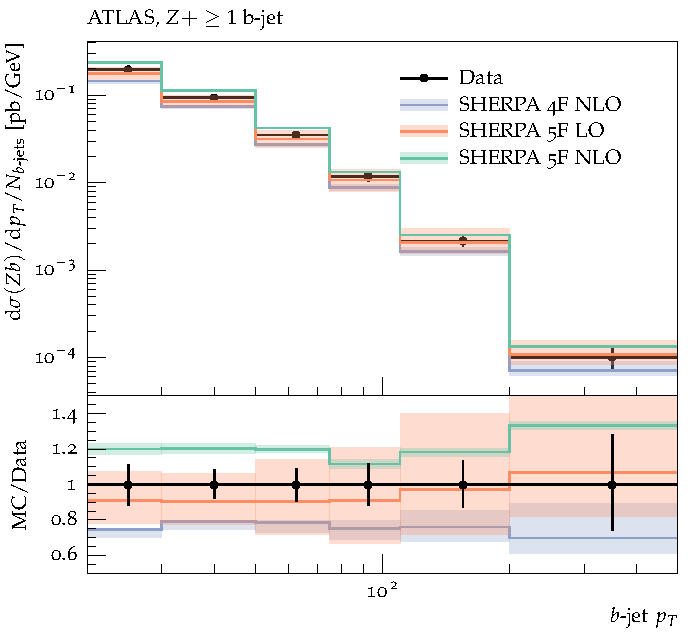
\includegraphics[scale=0.5]{figs/zbb/d03-x01-y01.pdf} 
   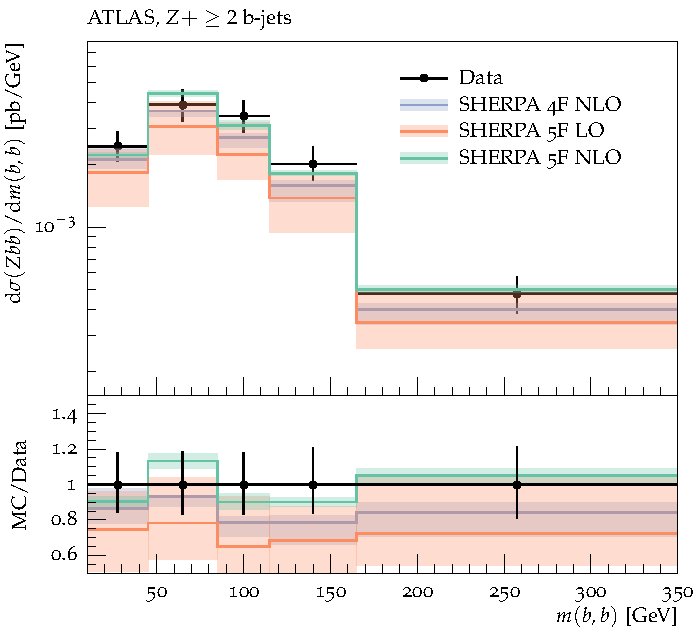
\includegraphics[scale=0.5]{figs/zbb/d23-x01-y01.pdf} 
\end{figure}
\begin{figure}[htbp]
   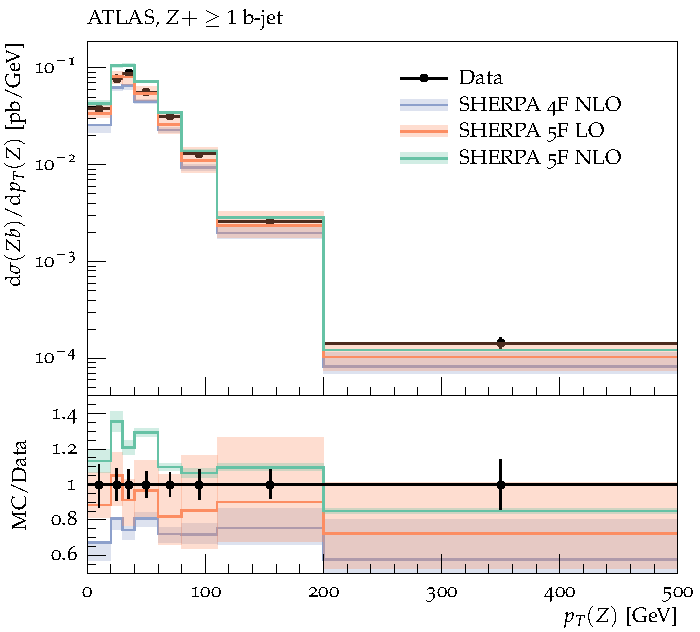
\includegraphics[scale=0.5]{figs/zbb/d15-x01-y01.pdf} 
   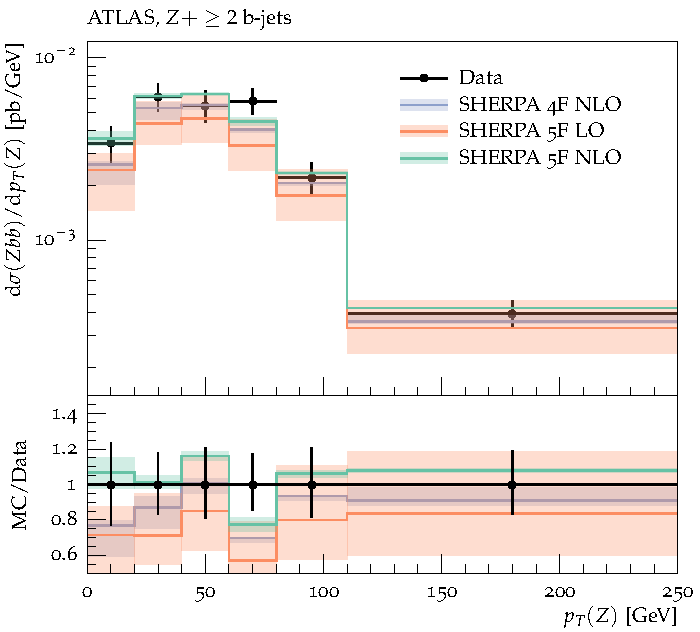
\includegraphics[scale=0.5]{figs/zbb/d25-x01-y01.pdf} 
\end{figure}
\begin{figure}[htbp]
   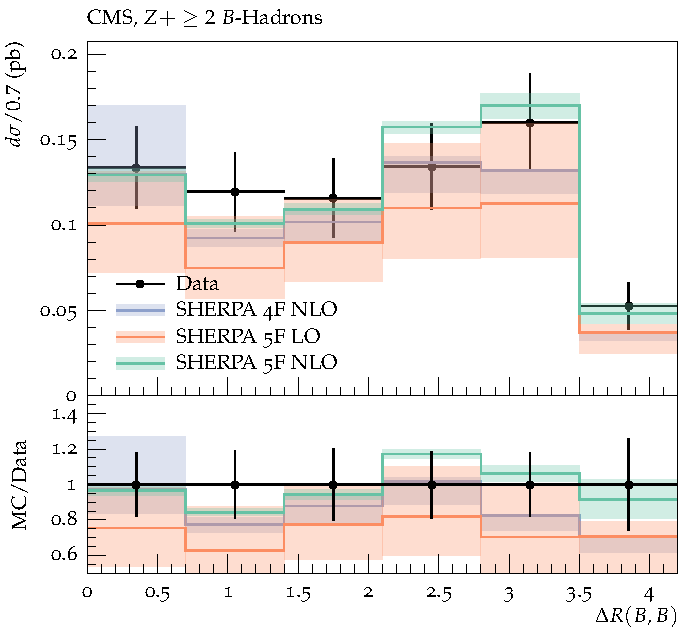
\includegraphics[scale=0.5]{figs/zbb/d01-x01-y01.pdf} 
   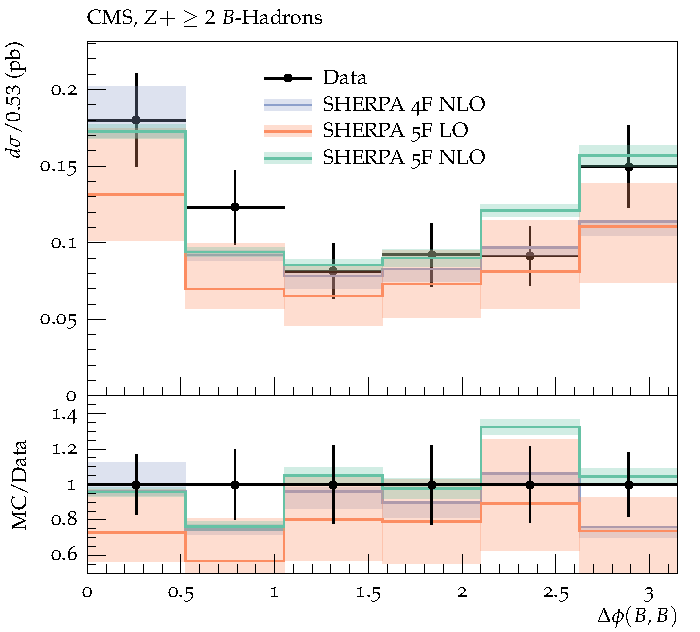
\includegraphics[scale=0.5]{figs/zbb/d02-x01-y01.pdf} 
\end{figure}
\subsubsection{Z+b 4F rescaled results}
...4F \MCatNLO rescaled to MCFM...
\begin{figure}[htbp]
   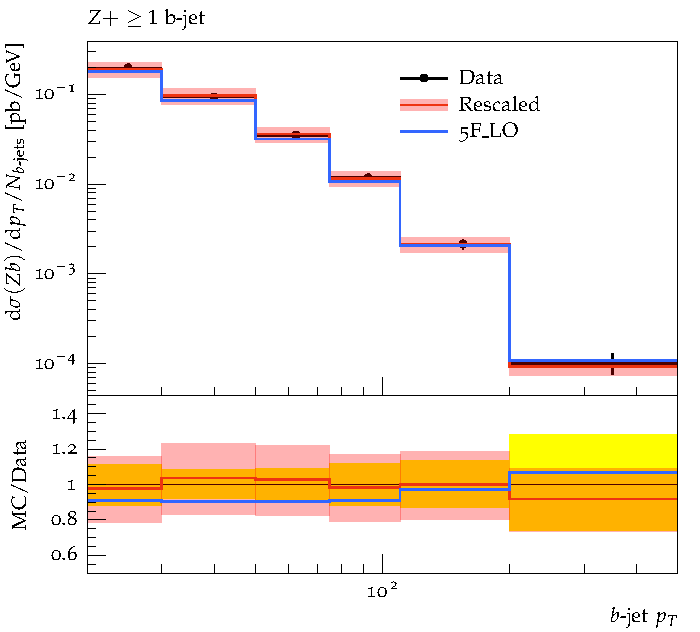
\includegraphics[scale=0.5]{figs/zbb/d03-x01-y01_rescaled.pdf} 
   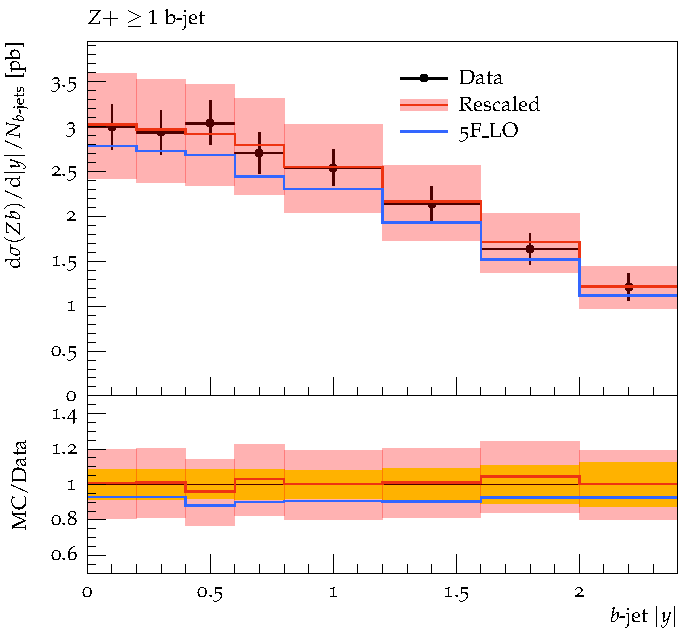
\includegraphics[scale=0.5]{figs/zbb/d05-x01-y01_rescaled.pdf} 
\end{figure}
\begin{figure}[htbp]
   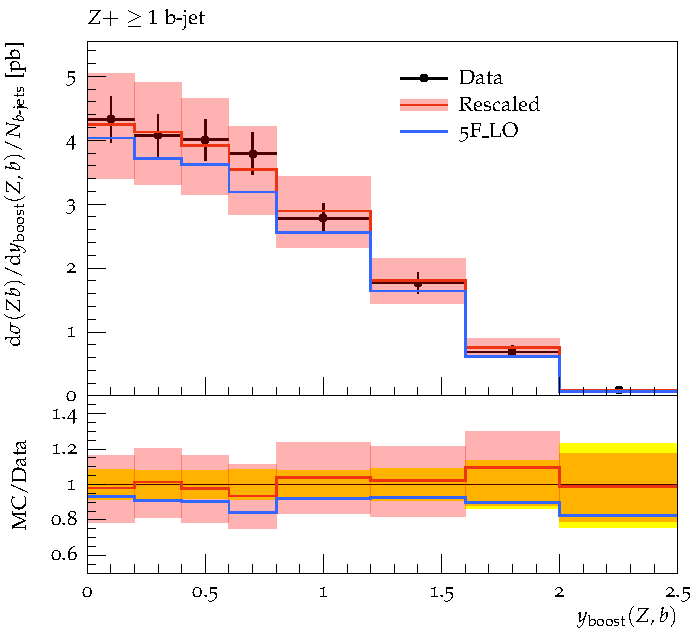
\includegraphics[scale=0.5]{figs/zbb/d07-x01-y01_rescaled.pdf} 
   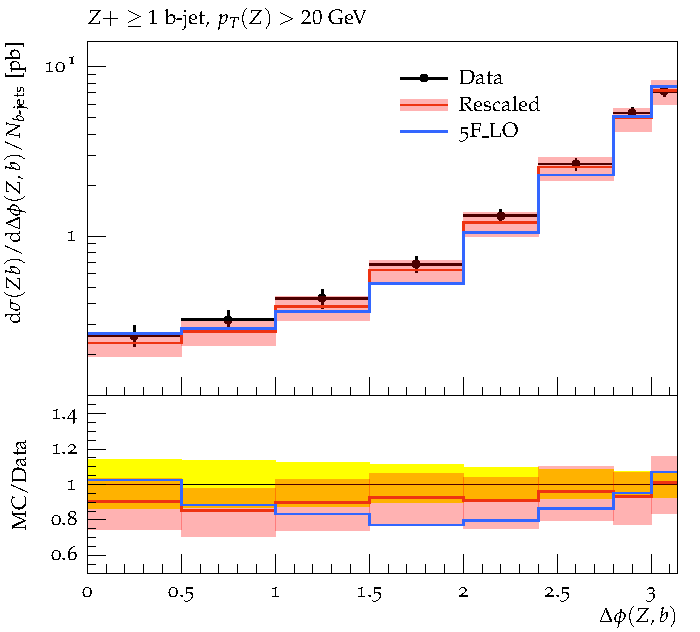
\includegraphics[scale=0.5]{figs/zbb/d11-x01-y01_rescaled.pdf} 
\end{figure}
\begin{figure}[htbp]
   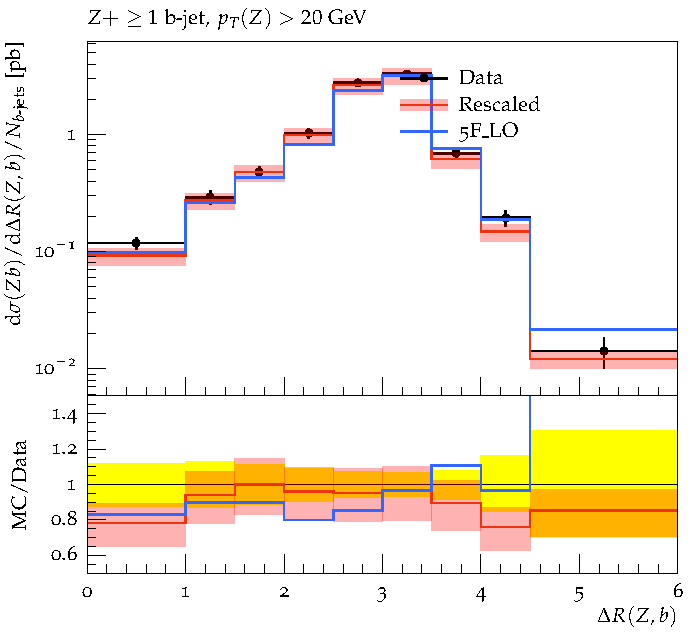
\includegraphics[scale=0.5]{figs/zbb/d13-x01-y01_rescaled.pdf} 
\end{figure}

\subsection{W+b production}

\subsection{Conclusions}

\bibliography{Vbb}

\end{document}
